\let\negmedspace\undefined
\let\negthickspace\undefined
\documentclass[journal]{IEEEtran}
\usepackage[a5paper, margin=10mm, onecolumn]{geometry}
\usepackage{tfrupee}

\setlength{\headheight}{1cm}
\setlength{\headsep}{0mm}

\usepackage{gvv-book}
\usepackage{gvv}
\usepackage{cite}
\usepackage{amsmath,amssymb,amsfonts,amsthm}
\usepackage{algorithmic}
\usepackage{graphicx}
\usepackage{textcomp}
\usepackage{xcolor}
\usepackage{txfonts}
\usepackage{listings}
\usepackage{enumitem}
\usepackage{mathtools}
\usepackage{gensymb}
\usepackage{comment}
\usepackage[breaklinks=true]{hyperref}
\usepackage{tkz-euclide}
\usepackage{listings}
\def\inputGnumericTable{}
\usepackage[latin1]{inputenc}
\usepackage{color}
\usepackage{array}
\usepackage{longtable}
\usepackage{calc}
\usepackage{multirow}
\usepackage{hhline}
\usepackage{ifthen}
\usepackage{lscape}

\begin{document}

\bibliographystyle{IEEEtran}
\vspace{3cm}

\title{4.5.5}
\author{EE25BTECH11003 - Adharvan Kshathriya Bommagani}
{\newpage\maketitle}

\renewcommand{\thefigure}{\theenumi}
\renewcommand{\thetable}{\theenumi}
\setlength{\intextsep}{10pt}

\textbf{Question}:\\
Find the vector equation of the line which is parallel to the vector $3\hat{i} - 2\hat{j} + 6\hat{k}$ and passes through the point $(1, -2, 3)$.

\bigskip

\textbf{Solution}:\\

The vector equation of a line is given by the formula:
$$ \vec{x} = \vec{h} + t\vec{m} $$
where:

    \textbf{$\vec{x}$} is the position vector of any point on the line, represented as $\myvec{x \\ y \\ z}$.\\
    \textbf{$\vec{h}$} is the position vector of a known point on the line.\\
    \textbf{$\vec{m}$} is the direction vector of the line.\\
    \textbf{$t$} is a scalar parameter.\\



The problem states that the line passes through the point $(1, -2, 3)$. The position vector for this point is:
\begin{align*}
\vec{h} = \myvec{1 \\ -2 \\ 3}
\end{align*}


The problem states that the line is parallel to the vector $3\hat{i} - 2\hat{j} + 6\hat{k}$. This is the direction vector of the line:
\begin{align*}
\vec{m} = \myvec{3 \\ -2 \\ 6}
\end{align*}


Now, substitute the vectors $\vec{h}$ and $\vec{m}$ into the general equation $\vec{x} = \vec{h} + t\vec{m}$.
The vector equation of the line is:
\begin{align*}
\myvec{x \\ y \\ z} = \myvec{1 \\ -2 \\ 3} + t \myvec{3 \\ -2 \\ 6}
\end{align*}

\bigskip

The vector equation of the line is:
$$ \myvec{x \\ y \\ z} = \myvec{1 \\ -2 \\ 3} + t \myvec{3 \\ -2 \\ 6} $$



\textbf{Plot of the Line:}
\begin{figure}[h!]
    \centering
    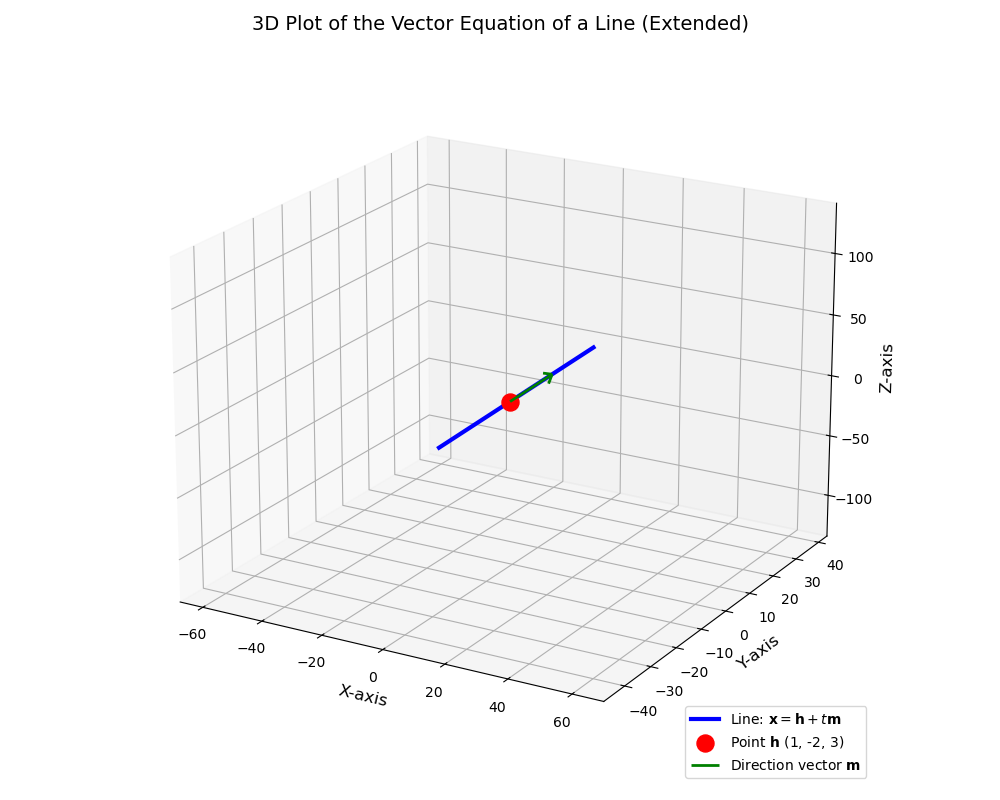
\includegraphics[width=1.0\columnwidth]{figs/fig1.png}
    \caption{Figure for 4.5.5}
    \label{}
\end{figure}

\end{document}